\chapter{Podstawy teoretyczne}

Celem rozdziału jest przedstawienie podstawowych definicji, wytłumaczenie aparatu matematycznego oraz metod wykorzystywanych w algorytmach na których skupia się praca. Dodatkowo ma on na celu ułatwienie dalszego czytania poprzez zapoznanie czytelnika z przyjętymi konwencjami, oznaczeniami oraz symbolami, które mogą pojawić się w kolejnych rozdziałach. 


\section{Definicja super-rozdzielczości}

Super-rozdzielczość (ang. Super-Resolution) odnosi się do procesu poprawy rozdzielczości obrazu lub sekwencji obrazów. W kontekście cyfrowym, super-rozdzielczość jest często realizowana za pomocą algorytmów komputerowych, które mają na celu odtworzenie wysokiej rozdzielczości obrazu [Rys \ref{fig:image2}, \ref{fig:image3}] z jednego lub wielu obrazów o niskiej rozdzielczość [Rys \ref{fig:image1}].

\begin{figure}[ht]
    \centering
    \begin{minipage}[t]{0.3\linewidth}
        
\includegraphics[width=\linewidth]{Rozdziały/02.Podstawy_teoretyczne/comic.png}
        \caption{Obraz oryginalny}
        \label{fig:image1}
    \end{minipage}
    \hspace{0.5cm}
    \begin{minipage}[t]{0.3\linewidth}
        
\includegraphics[width=\linewidth]{Rozdziały/02.Podstawy_teoretyczne/comic_ESRGAN_x4.png}
        \caption{Obraz powiększony czterokrotnie}
        \label{fig:image2}
    \end{minipage}
    \hspace{0.5cm}
    \begin{minipage}[t]{0.3\linewidth}
        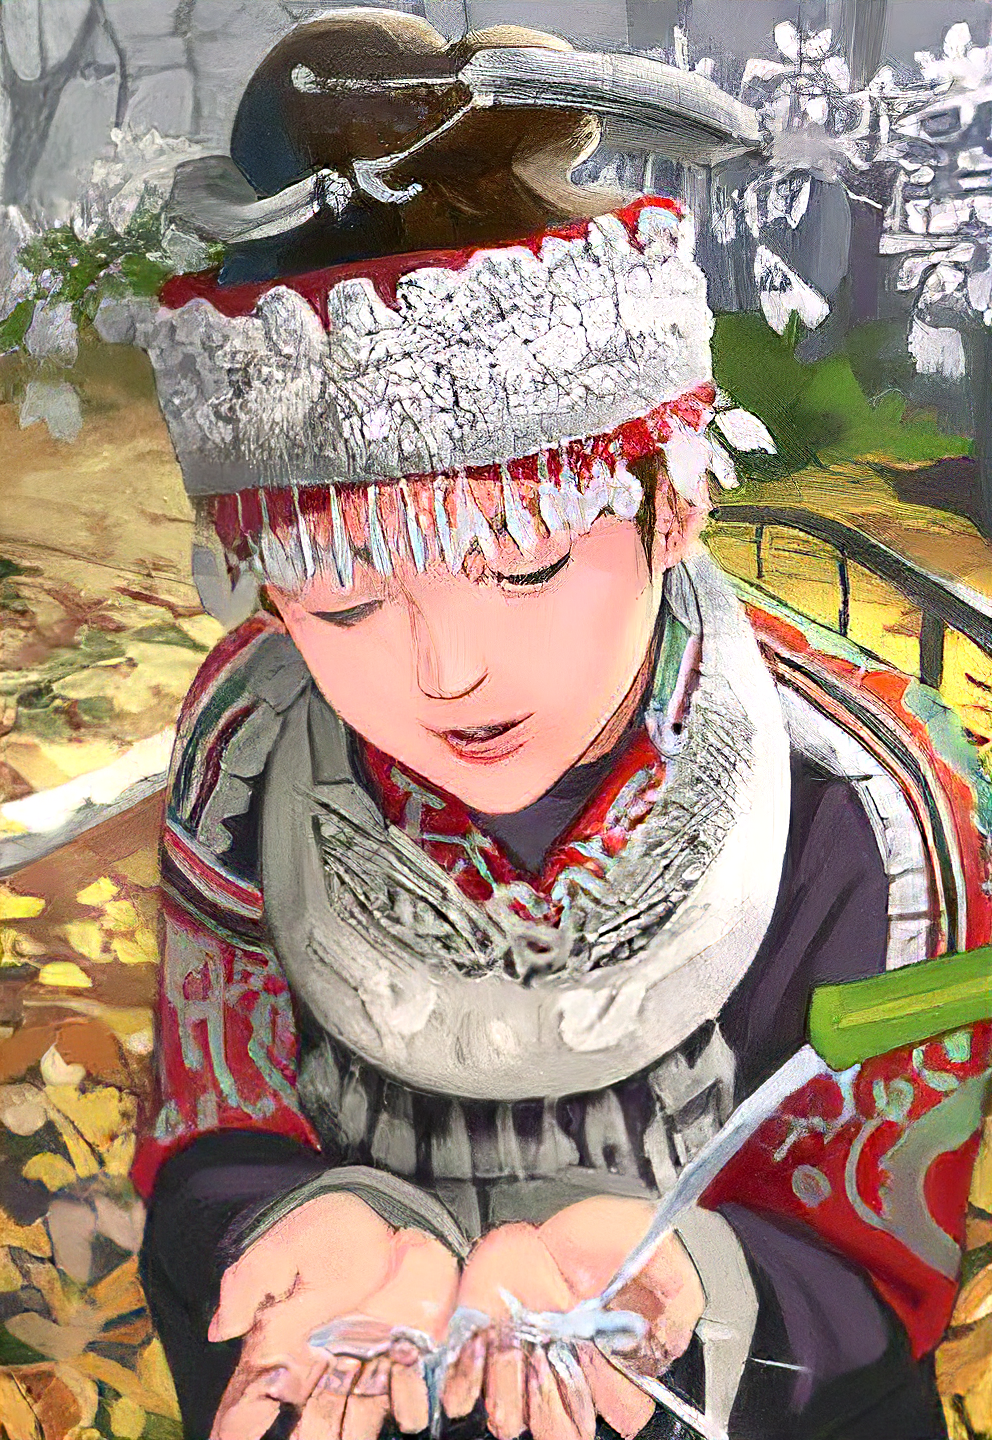
\includegraphics[width=\linewidth]{Rozdziały/02.Podstawy_teoretyczne/comic_ESRGAN_x16.png}
        \caption{Obraz powiększony szesnastokrotnie}
        \label{fig:image3}
    \end{minipage}
\end{figure}

\subsection*{Przykłady zastosowań super-rozdzielczości}

W kontekście praktycznym, techniki super-rozdzielczości znalazły zastosowanie w wielu dziedzinach. Przykładowo, w medycynie, poprawa rozdzielczości obrazów rentgenowskich może znacząco wpływać na dokładność diagnoz. W branży rozrywkowej, technika ta umożliwia remastering starych gier, filmów czy materiałów wideo do standardów HD czy 4K.

W ostatnich miesiącach popularne stało się generowanie obrazów z użyciem sztucznej inteligencji na podstawie podanego opisu tekstowego. Generowane w ten sposób obrazy są określonej wielkości i popularne modele takie jak \textbf{DALL-E} czy \textbf{Midjourney} nie pozwalają na zwiększenie jej. W tym miejscu z pomocą przychodzi super-rozdzielczość, która pozwala na powiększenie obrazu.


\section{Przegląd metod powiększania obrazów}


Istnieje wiele metod powiększania rozdzielczości obrazów. Najprostszą z nich jest \textbf{interpolacja najbliższego sąsiada}, która polega na powieleniu pobliskich pikseli w celu zwiększenia rozdzielczości obrazu. \\
Metoda ta jest bardzo prosta w implementacji, jednakże nie daje ona zadowalających rezultatów. Obraz powiększony w ten sposób wygląda jak obraz o niskiej rozdzielczości z większymi pikselami [Rys \ref{fig:image5}]. 

\begin{figure}[ht]
    \centering
    \begin{minipage}[t]{0.32\linewidth}
        
\includegraphics[width=\linewidth]{Rozdziały/02.Podstawy_teoretyczne/comic.png}
        \caption{Obraz oryginalny}
        \label{fig:image4}
    \end{minipage}
    \hspace{0.5cm}
    \begin{minipage}[t]{0.32\linewidth}
        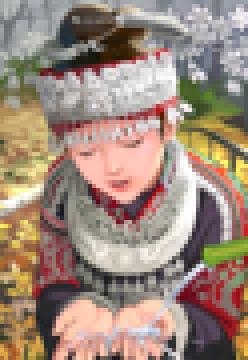
\includegraphics[width=\linewidth]{Rozdziały/02.Podstawy_teoretyczne/comic_NN_x4.png}
        \caption{Obraz powiększony metodą najbliższego sąsiada}
        \label{fig:image5}
    \end{minipage}
  \end{figure}


Aby poprawić jakość obrazu, można zastosować \textbf{interpolację dwuliniową}. Metoda ta rozszerza interpolację liniową na interpolację funkcji dwóch zmiennych [Rys \ref{fig:image6}]. 

\begin{figure}[ht]
    \centering
    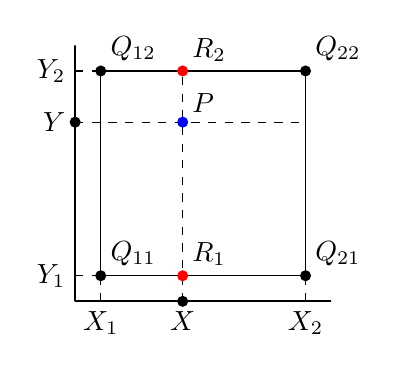
\begin{tikzpicture}[scale=1.3, dot/.style={circle,fill=black,minimum size=4pt,inner sep=0pt,outer sep=-1pt},]

        % Define the coordinates of the grid points
        \coordinate (A) at (1,1);
        \coordinate (B) at (3,1);
        \coordinate (C) at (1,3);
        \coordinate (D) at (3,3);

        \coordinate (R1) at (1.8,1);
        \coordinate (RY) at (1,2.5);
        \coordinate (R1end) at (1.8,3);
        \coordinate (RYend) at (3,2.5);

        \coordinate (P) at (1.8,2.5);

        \coordinate (X) at (1.8,0.75);
        \coordinate (Y) at (0.75,2.5);
        \coordinate (X1) at (1,0.75);
        \coordinate (X2) at (3,0.75);
        \coordinate (Y1) at (0.75,1);
        \coordinate (Y2) at (0.75,3);
        
        \coordinate (frameS) at (0.75,0.75);
        \coordinate (frameX) at (3.25,0.75);
        \coordinate (frameY) at (0.75,3.25);


        \draw[thick] (frameS) rectangle (frameX);
        \draw[thick] (frameS) rectangle (frameY);
        
        \draw[thin] (A) rectangle (D);
        
        % Draw lines from corners to the interpolated point
        \draw[dashed] (X) -- (R1end);
        \draw[dashed] (Y) -- (RYend);
        \draw[dashed] (X1) -- (A);
        \draw[dashed] (X2) -- (B);
        \draw[dashed] (Y1) -- (A);
        \draw[dashed] (Y2) -- (C);

        % Draw the dots
        \node[dot] at (A) {};
        \node[dot] at (B) {};
        \node[dot] at (C) {};
        \node[dot] at (D) {};
        \node[dot, blue] at (P) {};
        \node[dot, red] at (R1) {};
        \node[dot, red] at (R1end) {};
        \node[dot] at (X) {};
        \node[dot] at (Y) {};
        
        % Labels for the corners
        \node[above right] at (A) {$Q_{11}$};
        \node[above right] at (B) {$Q_{21}$};
        \node[above right] at (C) {$Q_{12}$};
        \node[above right] at (D) {$Q_{22}$};
        
        % Label for the interpolated point
        \node[above right] at (P) {$P$};

        \node[above right] at (R1) {$R_{1}$};
        \node[above right] at (R1end) {$R_{2}$};
        \node[below] at (X) {$X$};
        \node[left] at (Y) {$Y$};
        \node[below] at (X1) {$X_{1}$};
        \node[below] at (X2) {$X_{2}$};
        \node[left] at (Y1) {$Y_{1}$};
        \node[left] at (Y2) {$Y_{2}$};
        

        % Add title
        % \node[below] at (current bounding box.south) {Wizualizacja interpolacji dwuliniowej};

    \end{tikzpicture}
    \caption{Wizualizacja interpolacji dwuliniowej}
    \label{fig:image6}
\end{figure}


W efekcie polega to na wyznaczeniu średniej ważonej pikseli sąsiadujących z pikselem, który chcemy powielić. Współczynniki wag są wyznaczane na podstawie odległości od piksela, który chcemy powielić.
Kroki algorytmu:
\begin{enumerate}
    \item Przeprowadzana jest interpolacja liniowa wzdłuż osi $O X$:
    
    $$
    \begin{array}{llll}
    f\left(R_1\right) \approx \frac{x_2-x}{x_2-x_1} f\left(Q_{11}\right)+\frac{x-x_1}{x_2-x_1} f\left(Q_{21}\right) & \text { gdzie } & R_1=\left(x, y_1\right), \\ \\
    f\left(R_2\right) \approx \frac{x_2-x}{x_2-x_1} f\left(Q_{12}\right)+\frac{x-x_1}{x_2-x_1} f\left(Q_{22}\right) & \text { gdzie } & R_2=\left(x, y_2\right) .
    \end{array}
    $$
    \item Następnie przeprowadzana jest interpolacja wzdłuż osi $O Y$:
    $$
    f(P) \approx \frac{y_2-y}{y_2-y_1} f\left(R_1\right)+\frac{y-y_1}{y_2-y_1} f\left(R_2\right) .
    $$
\end{enumerate}


W efekcie otrzymujemy obraz wyglądający następująco [Rys \ref{fig:image8},  \ref{fig:image10}].


\begin{figure}[ht]
    \centering
    \begin{minipage}[t]{0.33\linewidth}
        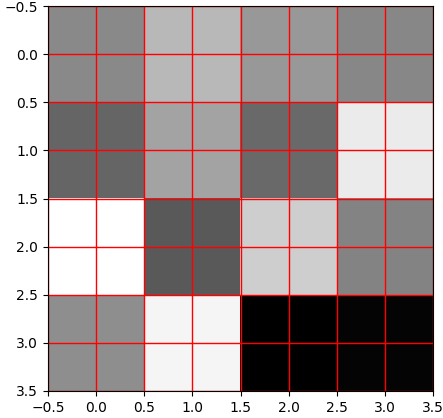
\includegraphics[width=\linewidth]{Rozdziały/02.Podstawy_teoretyczne/bilinear_original.png}
        \caption{Obraz wejściowy}
        \label{fig:image7}
    \end{minipage}
    \hspace{0.5cm}
    \begin{minipage}[t]{0.33\linewidth}
        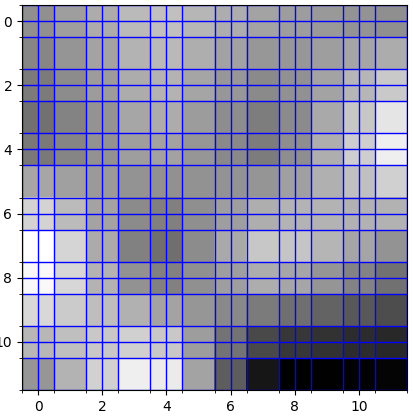
\includegraphics[width=\linewidth]{Rozdziały/02.Podstawy_teoretyczne/bilinear_enlarged.png}
        \caption{Obraz powiększony przez interpolację dwuliniową}
        \label{fig:image8}
    \end{minipage}
\end{figure}

\begin{figure}[ht]
    \centering
    \begin{minipage}[t]{0.33\linewidth}
        
\includegraphics[width=\linewidth]{Rozdziały/02.Podstawy_teoretyczne/comic.png}
        \caption{Obraz wejściowy}
        \label{fig:image9}
    \end{minipage}
    \hspace{0.5cm}
    \begin{minipage}[t]{0.33\linewidth}
        
\includegraphics[width=\linewidth]{Rozdziały/02.Podstawy_teoretyczne/comic_BILINEARx4.png}
        \caption{Obraz powiększony przez interpolację dwuliniową}
        \label{fig:image10}
    \end{minipage}
\end{figure}


Metoda ta daje lepsze rezultaty niż interpolacja najbliższego sąsiada, jednakże wprowadziła ona duże rozmycie, które jest szczególnie widoczne na krawędziach obiektów i obszarach wysokiej częstotliwości.

\subsection*{Teoria informacji}

W teorii informacji istnieje koncepcja zwana \textbf{nierównością przetwarzania danych}. Zgodnie z nią niezależnie od sposobu przetwarzania danych, \textbf{nie można dodać informacji, której nie ma w oryginalnej serii danych}  [Wzór 2.1].

\begin{equation}
    \begin{gathered}
    X \rightarrow Y \rightarrow Z \\
    I(X ; Y) \geq I(X ; Z)
    \end{gathered}
\end{equation}

Oznacza to, że brakujących danych nie można odzyskać poprzez dalsze przetwarzanie. Czy to oznacza, że super-rozdzielczość jest teoretycznie niemożliwa? 

Nie, jeśli mamy dodatkowe źródło informacji. 


% \newpage
\section{Wprowadzenie do głębokiego uczenia się w przetwarzaniu obrazów}

Głębokie uczenie rewolucjonizuje przetwarzanie obrazów, wprowadzając modele zdolne do uczenia się cech z serii danych. W przetwarzaniu obrazów, głębokie sieci neuronowe są wykorzystywane do zadań takich jak detekcja obiektów, segmentacja, klasyfikacja obrazów, czy właśnie super-rozdzielczość [Rys \ref{fig:image12},  \ref{fig:image13}].

\begin{figure}[ht]
    \centering
    \begin{minipage}[t]{0.3\linewidth}
        
\includegraphics[width=\linewidth]{Rozdziały/02.Podstawy_teoretyczne/comic.png}
        \caption{Obraz wejściowy}
        \label{fig:image11}
    \end{minipage}
    \hspace{0.5cm}
    \begin{minipage}[t]{0.3\linewidth}
        
\includegraphics[width=\linewidth]{Rozdziały/02.Podstawy_teoretyczne/comic_DWSR_x4.png}
        \caption{Obraz powiększony algorytmem DWSR}
        \label{fig:image12}
    \end{minipage}
    \hspace{0.5cm}
    \begin{minipage}[t]{0.3\linewidth}
        
\includegraphics[width=\linewidth]{Rozdziały/02.Podstawy_teoretyczne/comic_ESRGAN_x4.png}
        \caption{Obraz powiększony algorytmem ESRGAN}
        \label{fig:image13}
    \end{minipage}
\end{figure}

Sieć neuronowa może nauczyć się odtwarzać szczegóły obrazów na podstawie pewnych informacji, które zbiera z dużego zbioru obrazów. 

Szczegóły dodawane do powiększanego obrazu w przy użyciu modelu uczenia maszynowego nie naruszają nierówności przetwarzania danych, ponieważ wykorzystywane informacje są w zbiorze treningowym, nawet jeśli nie ma ich na obrazie wejściowym.





\subsection*{Podstawy Głębokiego Uczenia}
Głębokie uczenie, będące zaawansowaną formą uczenia maszynowego, wykorzystuje wielowarstwowe sieci neuronowe do analizy i interpretacji dużych zbiorów danych. Te sieci składają się z warstw skomplikowanych struktur algorytmicznych, które naśladują sposób, w jaki ludzki mózg przetwarza informacje.


\subsubsection*{Architektura Sieci Neuronowych}
Architektura sieci neuronowych w głębokim uczeniu charakteryzuje się wieloma ukrytymi warstwami, które pozwalają na przetwarzanie danych na różnych poziomach abstrakcji. Każda warstwa składa się z wielu neuronów, z których każdy otrzymuje dane wejściowe, przetwarza je i przekazuje dalej. Istnieją różne rodzaje warstw, w tym:
\begin{itemize}
    \item \textbf{Warstwy konwolucyjne (Convolutional Layers)}: Są fundamentem sieci konwolucyjnych (CNNs), które są szeroko stosowane w przetwarzaniu obrazów. Te warstwy stosują filtr konwolucyjny do danych wejściowych, wydobywając lokalne cechy, takie jak krawędzie, kształty czy tekstury.
    \item \textbf{Warstwy pooling (Pooling Layers)}: Redukują wymiarowość danych, jednocześnie zachowując ważne informacje. Najczęściej stosowanymi są max pooling i average pooling.
    \item \textbf{Warstwy w pełni połączone (Fully Connected Layers)}: Każdy neuron w tych warstwach jest połączony ze wszystkimi neuronami w poprzedniej warstwie, co pozwala na integrację nauczonej wiedzy z poprzednich warstw.
\end{itemize}


\subsubsection*{Funkcje Aktywacji}
Funkcje aktywacji w sieciach neuronowych to nieliniowe transformacje stosowane do wyjść neuronów. Decydują one o tym, czy dany neuron zostanie aktywowany, czyli czy jego informacje zostaną przekazane dalej. Najpopularniejsze funkcje aktywacji to:
\begin{itemize}
    \item \textbf{ReLU (Rectified Linear Unit)}: Przekształca wszystkie ujemne wartości na zero, podczas gdy wartości dodatnie pozostają niezmienione  [Rys \ref{fig:image14}].
    \item \textbf{Sigmoid}: Przyjmuje wartości wejściowe i konwertuje je na wartości z zakresu od 0 do 1 [Rys \ref{fig:image15}].
    \item \textbf{Tanh (Hyperbolic Tangent)}: Podobnie jak sigmoid, ale konwertuje wartości na zakres od -1 do 1 [Rys \ref{fig:image16}].
\end{itemize}

\begin{figure}[ht]
    \centering
    \begin{minipage}[t]{0.3\linewidth}
        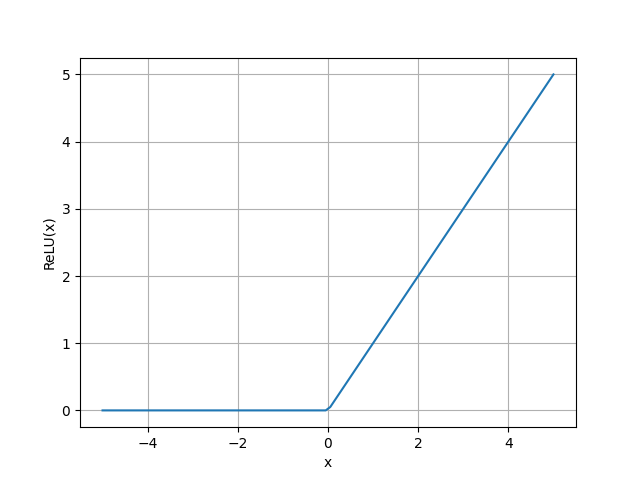
\includegraphics[width=\linewidth]{Rozdziały/02.Podstawy_teoretyczne/relu.png}
        \caption{ReLU}
        \label{fig:image14}
    \end{minipage}
    \hspace{0.5cm}
    \begin{minipage}[t]{0.3\linewidth}
        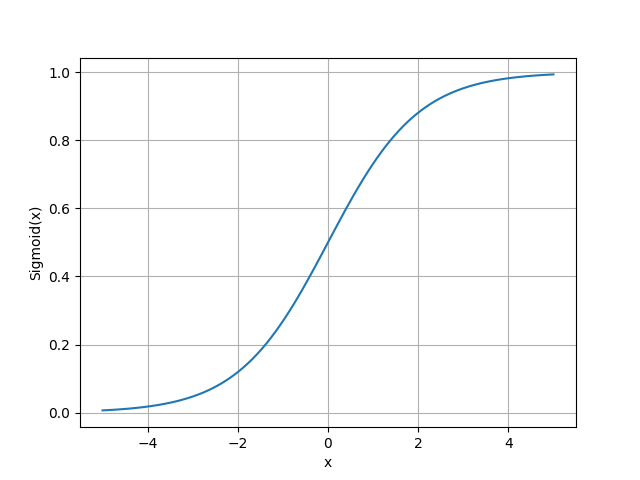
\includegraphics[width=\linewidth]{Rozdziały/02.Podstawy_teoretyczne/sigmoid.png}
        \caption{Sigmoid}
        \label{fig:image15}
    \end{minipage}
    \hspace{0.5cm}
    \begin{minipage}[t]{0.3\linewidth}
        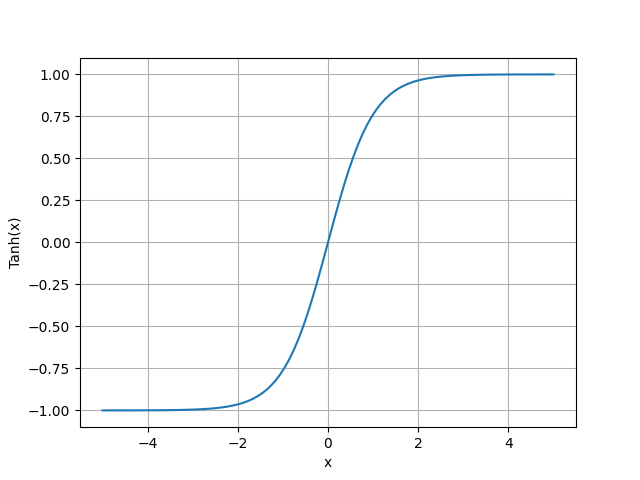
\includegraphics[width=\linewidth]{Rozdziały/02.Podstawy_teoretyczne/tanh.png}
        \caption{anh}
        \label{fig:image16}
    \end{minipage}
\end{figure}


\subsubsection*{Proces Uczenia}


\subsubsection*{Przeuczenie i Generalizacja}



\subsection*{Algorytmy Głębokiego Uczenia w Super-Rozdzielczości}

W tej pracy opisywane będą szczegółowo dwa bardzo ciekawe algorytmy głębokiego uczenia stosowane w zadaniu super-rozdzielczości. Jeden z nich wykorzystuje 



\newpage
\section{Wstęp do funkcji falkowych}


Omówienie funkcji falkowych, opis do czego to narzędzie służy począwszy od transformaty Fouriera i jej ograniczeń, 
w jaki sposób funkcje falkowe rozwijają FFT, przedstawienie działania.





% \newpage
% \section*{Chatbot:}

% \section*{Przegląd metod powiększania obrazów}

% Tradycyjne metody powiększania obrazów obejmują interpolację najbliższego sąsiada, interpolację dwuliniową oraz interpolację dwusześcienną. Te techniki opierają się na prostych przekształceniach matematycznych i mogą być łatwo implementowane, lecz często prowadzą do efektów ubocznych takich jak rozmycie czy artefakty.

% Współczesne techniki wykorzystują bardziej zaawansowane podejścia, takie jak rekonstrukcja oparta na przykładowych obrazach (example-based reconstruction), gdzie wykorzystuje się zbiór danych zawierający pary obrazów LR i HR, aby nauczyć algorytm odtwarzania szczegółów na wysokim poziomie rozdzielczości. Metody te mogą wykorzystywać różnorodne techniki, w tym mapowanie cech, modelowanie statystyczne, a nawet uczenie maszynowe.

% W ostatniej dekadzie, z uwagi na rozwój w dziedzinie uczenia maszynowego, pojawiły się metody bazujące na głębokich sieciach neuronowych, takie jak konwolucyjne sieci neuronowe (CNN, z ang. Convolutional Neural Networks) w zadaniach SR. Przykładami takich metod są SRCNN (Super-Resolution Convolutional Neural Network), VDSR (Very Deep Super-Resolution), EDSR (Enhanced Deep Super-Resolution) oraz GAN (Generative Adversarial Networks) wykorzystywane w modelu SRGAN (Super-Resolution Generative Adversarial Network), które przynoszą znaczące ulepszenia w jakości rekonstruowanych obrazów HR.
 
% \section*{Wprowadzenie do głębokiego uczenia się w przetwarzaniu obrazów}



% Podstawową jednostką w konwolucyjnych sieciach neuronowych jest warstwa konwolucyjna, która skanuje obraz za pomocą filtrów (również nazywanych jądrami), wyodrębniając lokalne cechy. Następnie, warstwy pooling redukują wymiarowość danych, zachowując przy tym najważniejsze informacje. Głębokie sieci neuronowe mogą składać się z wielu takich warstw, co pozwala na wyodrębnianie coraz bardziej abstrakcyjnych cech z obrazów.

% Sieci te są trenowane przy użyciu zestawów danych, gdzie algorytm uczy się mapowania między danymi wejściowymi a oczekiwanymi wynikami. W zadaniach SR, sieć jest trenowana do przewidywania obrazów HR z obrazów LR, przy czym jakość wyniku jest oceniana przy pomocy funkcji straty, takiej jak błąd średniokwadratowy (MSE, z ang. Mean Squared Error) czy wskaźnik strukturalnej jakości obrazu (SSIM, z ang. Structural Similarity Index).

% Nowoczesne podejścia do SR często wykorzystują także sieci GAN, które składają się z dwóch części: generatora, który generuje obrazy, oraz dyskryminatora, który ocenia, czy obrazy są wystarczająco zbliżone do prawdziwych HR. Konkurencyjna dynamika między tymi dwoma sieciami prowadzi do generowania coraz lepszych obrazów.

% W dalszych rozdziałach szczegółowo omówimy te techniki, przedstawiając zarówno ich teoretyczne podstawy, jak i praktyczne zastosowania. Zostaną przedstawione również aktualne wyzwania i kierunki badań w dziedzinie super-rozdzielczości, co pozwoli czytelnikowi na głębsze zrozumienie tego dynamicznie rozwijającego się obszaru wiedzy.

% \section*{Youtube - super resolution}


% So, how can we train such a model?
% If you watched my Deep Learning Crash Course series, you might be thinking: can't we just
% train a neural network to learn a mapping between low and high-resolution images?
% Yes, we can, and we wouldn't be the first ones to do so.
% Dataset
% That's pretty much what the SRCNN paper did.
% First, we can create a dataset by collecting high-resolution images and downscaling them,
% or we can simply use one of the existing super-resolution datasets, such as the DIV2K dataset.
% Then, we can build a convolutional neural network that would input only the low-resolution
% images, and we can train it to produce higher resolution images that match the original
% ones the best.
% The SRCNN paper simply minimized the squared difference between the pixel values to produce
% images that are as close as possible to the original high-resolution images.
% Mean squared error
% But is mean squared error really the right metric to optimize?
% This is a very old debate.
% Long story short, mean squared error doesn't express the human perception of image fidelity
% well.
% For example, all of these distorted images are equally distant from the original image
% in terms of mean squared error.
% Clearly, they don't look equally good.
% Because mean squared error cares only about pixel-wise intensity differences but not the
% structural information about the contents of an image.
% There's a better measure of perceptual image quality called the structural similarity index,
% which was developed in my lab at the University of Texas at Austin.
% The structural similarity index made a very high impact, both in academia and the industry.
% My doctoral advisor, Alan Bovik, and his collaborators won a Primetime Emmy Award for this method
% a few years ago.
% This metric was initially developed to measure the severity of image degradations.
% However, many researchers also used it as a loss function to train neural networks for
% Perceptual loss
% image restoration.
% More recently, people also started using pre-trained convolutional neural networks as perceptually-relevant
% loss functions.
% How it works is that you first take a pre-trained model.
% This is typically a VGG-19 model trained on ImageNet.
% Then take it's first few layers and compute the difference between the feature maps produced
% by those layers.
% The difference between the feature maps can be minimized to train another model, just
% like any other loss function.
% The layers that generate those feature maps stay frozen during training and act as a fixed
% feature extractor.
% This method is commonly referred to as perceptual loss, content loss, or VGG-loss.
% How is this relevant to super-resolution?
% We can use this loss function to train models to enhance images and get pretty decent results.
% Super Resolution
% But, sometimes, it doesn't feel fair to penalize the model for pixelwise differences that don't
% really make much difference for human viewers.
% For example, does the direction of the hair on this baboon's face really matter?
% What if we cared a little less about how the original high-resolution images looked like,
% as long as the produced images looked good.
% We can do so by using GANs: generative adversarial networks.
% GANs consist of two networks fighting each other to achieve adversarial goals.
% I made a more detailed video about this earlier.
% There's a GAN-based super-resolution system called SRGAN.
% It uses a generator network that inputs low-resolution images and tries to produce their high-resolution
% versions.
% It also uses a discriminator network that tries to tell whether this is a real high-resolution
% image or an image upscaled by the generator.
% Both networks are trained simultaneously, and they both get better over time.
% Once the training is done, all we need is the generator part to upscale low-resolution
% images.
% In addition to this adversarial training setup, SRGAN also used a VGG-based loss function
% that we talked about earlier.
% There's another paper called Enhanced SRGAN, which proposed a few tricks to improve the
% ESR Gain
% results further.
% Enhanced SRGAN, or ESRGAN for short, somehow got popular in the gaming community.
% People started using it to upscale vintage games, and it worked pretty well.
% It's surprising how well it worked on video game graphics despite being trained only on
% natural images.
% Let's take a look at what enhancements the ESRGAN paper proposed for better results.
% First, they removed the batch normalization layers in their network architecture.
% This may sound contradictory to what I said in my previous videos, but it's not.
% Batch normalization does help a lot for many computer vision tasks.
% But for image-processing related tasks, such as super-resolution or image restoration in
% general, batch normalization can create some artifacts.
% They also added more layers and connections to their model architecture.
% It's not surprising that a more sophisticated model resulted in better images, but deeper
% models can be trickier to train, especially if they are not using batch normalization
% layers.
% So, the authors of ESRGAN used some tricks like residual scaling to stabilize the training
% of such a network.
% In addition to the changes in the model architecture, they also modified the loss functions.
% For example, they modified the VGG-loss in a way that compared the feature maps before
% activations.
% Their rationale is that the feature maps are denser and contain more information before
% they get clipped by the activation functions.
% In the original SRGAN paper, the discriminator model was trained to detect whether its input
% is real or fake.
% In the enhanced version, the authors used a relativistic discriminator that tells whether
% the input looks more realistic than fake data or less realistic than real data.
% Earlier I said minimizing the mean squared error might not be the best way to generate
% textures that look appealing to the human visual system.
% Then, I went on to say maybe we shouldn't care too much about how close the generated
% images are to the original ones.
% There's actually a trade-off there.
% Interpolation
% We would still want the upscaled images to be a faithful representation of the originals
% while having good-looking textures.
% The ESRGAN paper aims to find the sweet spot by interpolating between models.
% What they do is that they compute the weighted average of two models, one trained using mean
% squared error, and the other fine-tuned with adversarial training.
% Blending the parameters this way allows for finding the right balance between the two
% models without retraining them.
% Zoom to Learn
% More recently, another paper also explored the idea of network interpolation, and their
% results also look promising.
% Super-resolution is a relatively hot topic, and many researchers are experimenting with
% different ways of approaching this problem and are publishing their results.
% This paper, titled "Zoom to learn, Learn to zoom," for example, focuses on building a
% model that mimics optical zoom directly on raw sensor data.
% The authors created a dataset of raw images, and their corresponding optically zoomed ground
% truth.
% Super Resume
% They also proposed a loss function named "contextual bilateral loss" to handle slightly misaligned
% image pairs.
% Speaking of raw images, Google Pixel's Super Res Zoom feature showed that it's possible
% to achieve super-resolution through a burst of raw images.
% Google's method makes use of slight hand movements to fill in the missing spots in an upscaled
% image.
% So what if the user is using a tripod, and the image is perfectly still.
% Then, they deliberately jiggle the camera between the shots.
% So, to be able to implement this, you need to have complete control of the hardware.
% Single Frame Super Resolution
% Unlike the other methods we covered so far, Google's Super Res Zoom is a multi-frame super-resolution
% algorithm.
% If you don't have such bursts of images and want to upscale your pictures, you can easily
% use the single-frame super-resolution methods that we overviewed today.
% ESRGAN, for example, operates on a single input image and is very easy to run on an
% arbitrary picture you may want to use.
% Face Upscaling Super Resolution
% There are also task-specific super-resolution models, which I think is worth mentioning.
% For instance, face-upscaling models use face priors to synthesize realistic details on
% faces.
% Basically, the models know what a face typically looks like and uses that information to hallucinate
% the details.
% As you can tell, those methods are absolutely not suitable for CSI purposes, since all the
% details in the upscaled version are completely made up.
% Alright, that's all for today.
% I hope you liked it.
% I put the links to all referenced papers in the description below.
% Subscribe for more videos.
% And as always, thanks for watching, stay tuned, and see you next time.